\documentclass[a4paper, twocolumn]{article}

\usepackage[backend=biber]{biblatex}
\addbibresource{./refs.bib}

\usepackage{graphicx}
\usepackage{booktabs}
\usepackage{multirow}
\usepackage{float}
\usepackage{listings}
\usepackage{xcolor}
\usepackage[margin=2cm]{geometry}

\definecolor{lightgray}{gray}{0.9}

\lstset{
    showstringspaces=false,
    basicstyle=\ttfamily,
    keywordstyle=\color{blue},
    commentstyle=\color[gray]{0.6},
    stringstyle=\color[RGB]{255,150,75}
}

\newcommand{\inlinecode}[2]{\colorbox{lightgray}{\lstinline[language=#1]$#2$}}

\author{Aleksandr Sorokin, Viggo Beck, Sebastian Drumm, Hero Engelund} \title{Machine Learning on a small car dataset: Classification and Regression Analysis}

\begin{document}

\twocolumn[
    \begin{@twocolumnfalse}
        \maketitle
        \begin{abstract}
This project examines classification and regression tasks on a dataset of approximately 400 cars. Traditional machine learning models are used to predict car origin and engine horsepower. The results highlight challenges of small, imbalanced datasets and the importance of feature selection. 
        \end{abstract}
    \end{@twocolumnfalse}
]


\section{Introduction}
Machine learning models can be used to uncover patterns in structured datasets and make predictions based on observed relationships. In this project, we analyze a dataset containing various features of cars, including fuel efficiency, engine characteristics, and physical properties.

The goal is to formulate and solve two problems: a classification problem and a regression problem. Given the relatively small dataset size, careful model selection and regularization are necessary to avoid overfitting and ensure meaningful results.
\section{Problem Formulation}
\subsection{Classification Task}
We aim to answer the following research questions:
\begin{enumerate}
    \item To what extent can the origin of a car (1 = America, 2 = Europe, or 3 = Asia) be accurately predicted using features such as mpg, cylinders, horsepower, weight, acceleration, and model year?
    \item How do different models and hyperparameters choices affect classification performance on this dataset, especially given the class imbalance?
\end{enumerate}
\subsection{Regression Task}
The regression task aims to answer the following research questions:
\begin{enumerate}
    \item Which car attribute can be predicted most effectively from the available features?
    \item Which models and hyperparameter settings yield the best predictive performance for the selected target variable?
\end{enumerate}
\section{Methods}
We follow a structured Data Science process inspired by the principles for data analysis, emphasizing reproducibility and systematic workflows \cite{stoudt2021principles}.

\subsection{Data Preprocessing}
The dataset is imported using a fully scripted workflow to ensure reproducibility. Missing values (e.g., in horsepower) are handled through removal or imputation. Feature relationships are examined using correlation analysis to understand dependencies between variables.

\subsection{Model Selection and Hyperparameter Tuning}
Models are selected based on the dataset size and the nature of the task. Given the relatively small dataset, models that are robust to limited data and less prone to overfitting are preferred.

The selected models include Decision Tree, Random Forest, and Gradient Boosting for classification, and Linear Regression and Random Forest for regression. Hyperparameters are tuned using Randomized Search.
\subsection{Evaluation}
The dataset is split into training, validation and test sets to evaluate model performance. Classification performance is measured using accuracy and F1-score,  while regression performance is evaluated using RMSE and R-squared.
\section{Analysis}
Looking at the dataset, we found a class imbalance, meaning that roughly 60\% of the samples are American cars.

We did a correlation analysis using Pearson's R which revealed that some features, such as cylinders, showed limited predictive value and potential redundancy. 

Horsepower was selected as the regression target due to its strong correlation with multiple features, making it a more stable and predictable variable compared to acceleration.

For the regression task, feature scaling using StandardScaler was applied to account for differences in feature magnitudes.

For our classification task, we explored the data using box plots, here we found American cars are very distinct from Asian and European cars, for example as shown below on how many cylinders they have. 
\begin{figure}[H]
    \centering
    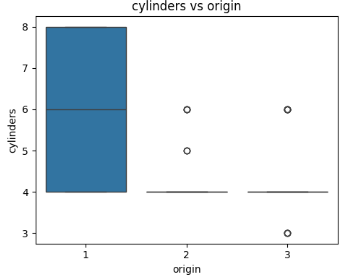
\includegraphics[width=\columnwidth]{image.png}
    \caption{Distribution of cylinders across car origins. }
    \label{fig:cylinders_origin}
\end{figure}

This will skew model performance in favor of American cars.
\section{Findings}
The analysis suggests that the formulation of the regression task has a substantial impact on model performance. In particular, predicting horsepower appears to be more feasible than predicting acceleration, as horsepower has stronger relationships with the features.
Below is the performance of our regression models, L = Linear Regression, R = Random Forest.
\begin{table}[H]
\centering
\caption{Regression Model Performance}
\begin{tabular}{l|l|c|c}
\hline
\textbf{Model} & \textbf{Dataset} & \textbf{R²} & \textbf{RMSE} \\
\hline
L& Train & 0.72 & 15.4 \\
 & Validation & 0.68 & 16.1 \\
 & Test & 0.69 & 15.8 \\
\hline
R& Train & 0.91 & 8.3 \\
 & Validation & 0.85 & 9.8 \\
 & Test & 0.87 & 9.1 \\
\hline
\end{tabular}
\label{tab:regression_results}
\end{table}
Below is the performance of our classification models, D = Decision Tree, R = Random Forest, G = Gradient Boosting.
\begin{table}[H]
\centering
\caption{Classification Model Performance}
\begin{tabular}{l|l|c|c}
\hline
\textbf{Model} & \textbf{Dataset} & \textbf{Accuracy} & \textbf{F1 Score} \\
\hline
D& Train & 1.00 & 1.00 \\
 & Validation & 0.82 & 0.82 \\
 & Test & 0.87 & 0.86 \\
\hline
R& Train & 0.95 & 0.95 \\
 & Validation & 0.77 & 0.77 \\
 & Test & 0.85 & 0.85 \\
\hline
G& Train & 1.00 & 1.00 \\
 & Validation & 0.83 & 0.83 \\
 & Test & 0.87 & 0.86 \\
\hline
\end{tabular}
\label{tab:classification_results}
\end{table}

Across both tasks, model performance was influenced by feature choice, preprocessing decisions, and hyperparameter settings. 

Below, we present the performance of a Random Forest Classifier on the test set, showing precision, recall, F1 score, and support for each car origin.

\begin{table}[H]
\centering
\caption{Classification Metrics by Class}
\begin{tabular}{c|c|c|c|c}
\hline
\textbf{Origin} & \textbf{Precision} & \textbf{Recall} & \textbf{F1 Score} \\
\hline
1 & 0.95 & 0.92 & 0.93 \\
2 & 0.62 & 0.80 & 0.70 \\
3 & 0.80 & 0.67 & 0.73 \\
\hline
\end{tabular}
\label{tab:class_metrics}
\end{table}

\section{Conclusion}
This project investigated both classification and regression tasks on a small car dataset, with the aim of answering specific research questions related to model performance and target selection.

For the classification task, the results show that it is possible to predict the origin of a car with relatively high accuracy using the selected features. However, model performance is influenced by both model choice and class imbalance, with some classes (particularly American cars) being easier to predict than others.

For the regression task, the analysis demonstrates that horsepower is a more suitable target variable than acceleration, due to its stronger relationships with the available features. In terms of model performance, the Random Forest regressor consistently outperformed the linear baseline, indicating that non-linear models are better suited for this task.

Overall, the findings highlight that both model selection and problem formulation play a critical role in achieving reliable results, especially when working with small datasets. The limited data size and class imbalance introduce uncertainty in the evaluation.

\begin{thebibliography}{9}

\bibitem{stoudt2021principles}
Stoudt, Sara, V{\'a}squez, V{\'a}leri N., and Martinez, Ciera C. 
\textit{Principles for data analysis workflows}. 
PLOS Computational Biology, 17(3): e1008770, 2021.

\end{thebibliography}

\end{document}